\title{DRUHG: \\Dialectical Reflection Universal Hierarchical Grouper}
\author{Pavel Artamonov\\Last of the Soviets\\\small{druhg.p@gmail.com}}
% https://github.com/artamono1/druhg/blob/master/papers/druhg_en.tex

\newcommand{\abstractText}{\noindent
We present a clustering method based on the philosophy of dialectical materialism. Data points self-develop into nested structures of different densities and capture global outliers. Druhg(\foreignlanguage{russian}{drug}) does not require any parameters that makes it a default choice in any data analysis.
\\This work immerses readers in a world of dialectics. It proposes a formalization of the dialectical method, but instead of the \textbf{idea}listic Hegelian triads reflecting of the Absolute Spirit, it uses the \textbf{mater}ialistic opposites of Being to Being reflections.

\textit{Keywords:} Clustering, Dialectics, Quantum Density, Mao, Hegel
}


%%%%%%%%%%%%%%%%%
% Configuration %
%%%%%%%%%%%%%%%%%

\documentclass[12pt, a4paper, twocolumn]{article}

\usepackage[utf8]{inputenc}
\usepackage{csquotes}
\usepackage[OT2, T1]{fontenc} % TODO: починить шрифты. Заменить T0 на T1 https:\\tex.stackexchange.com/questions/402626/default-font-rasterizes-very-badly-with-t1-fontenc
\usepackage[russian, english]{babel}

\setlength{\parskip}{.5em}
\newdimen\myvspace
\myvspace=.5em

\usepackage[
  %backend=biber, 
  natbib=true,
  style=numeric,
  sorting=none
]{biblatex}
\addbibresource{./druhg/druhg.bib}

\usepackage{soul} % this is for underlining with ul

\usepackage{xurl}
% \usepackage[super,comma,sort&compress]{natbib}
\usepackage[toc,page]{appendix}
\usepackage{algorithm}
\usepackage[noend]{algpseudocode}
\usepackage{abstract}
\usepackage{caption}
\usepackage{subcaption}
% \renewcommand{\thefigure}{\thesection.\arabic{figure}}
% \usepackage[figurename=Fig.]{caption}
% \renewcommand{\figurename}{Fig.}
\addto\captionsenglish{\renewcommand{\figurename}{Fig.}}
\renewcommand{\thesubfigure}{\arabic{subfigure}}

\usepackage{mathtools}
\usepackage{parskip}

\usepackage{rotating}
\usepackage{tabularray}% для таблиц
% \usepackage{multirow} 
% \usepackage{tabularx}

\usepackage{epigraph, varwidth}
% https://tex.stackexchange.com/questions/96650/width-of-epigraphs
% make epigraph size wary
\renewcommand{\epigraphsize}{\small}
\setlength{\epigraphwidth}{\linewidth}
\renewcommand{\textflush}{flushright}
\renewcommand{\sourceflush}{flushright}
% A useful addition
\newcommand{\epitextfont}{}
\newcommand{\episourcefont}{}

\makeatletter
\newsavebox{\epi@textbox}
\newsavebox{\epi@sourcebox}
\newlength\epi@finalwidth
\renewcommand{\epigraph}[2]{%
  \vspace{\beforeepigraphskip}
  {\epigraphsize\begin{\epigraphflush}
   \epi@finalwidth=\z@
   \sbox\epi@textbox{%
     \varwidth{1.05\epigraphwidth}
     \begin{\textflush}\epitextfont#1\end{\textflush}
     \endvarwidth
   }%
   \epi@finalwidth=\wd\epi@textbox
   \sbox\epi@sourcebox{%
     \varwidth{\epigraphwidth}
     \begin{\sourceflush}\episourcefont#2\end{\sourceflush}%
     \endvarwidth
   }%
   \ifdim\wd\epi@sourcebox>\epi@finalwidth 
     \epi@finalwidth=\wd\epi@sourcebox
   \fi
   \leavevmode\vbox{
     \hb@xt@\epi@finalwidth{\hfil\box\epi@textbox}
     \vskip1.75ex
     \hrule height \epigraphrule
     \vskip.75ex
     \hb@xt@\epi@finalwidth{\hfil\box\epi@sourcebox}
   }%
   \end{\epigraphflush}
   \vspace{\afterepigraphskip}}}
\makeatother
% end epigraph size

\usepackage{blindtext}
% \usepackage{draftwatermark}
% \SetWatermarkText{DRAFT}
% \SetWatermarkScale{2}
% \SetWatermarkColor[gray]{0.95}

\usepackage{graphicx}
\graphicspath{ {./druhg/} }
\newcommand{\githubPics}{https://raw.githubusercontent.com/artamono1/druhg/master/papers/druhg/}
\usepackage[export]{adjustbox}
% \usepackage{floatrow} % https://tex.stackexchange.com/questions/29143/caption-on-the-side-of-a-figure

\renewcommand{\abstractnamefont}{\normalfont\bfseries}
\renewcommand{\abstracttextfont}{\normalfont\small\itshape}
\usepackage{lipsum}
\usepackage{geometry}
\geometry{
 a4paper,
 total={170mm,257mm},
 left=20mm,
 top=20mm,
 right=15mm
}

%%%%%%%%%%%%%%
% References %
%%%%%%%%%%%%%%

% Any configuration that should be done before the end of the preamble:
\usepackage{hyperref}
\hypersetup{colorlinks=true, urlcolor=blue, linkcolor=blue, citecolor=blue}


\begin{document}

%%%%%%%%%%%%
% Abstract %
%%%%%%%%%%%%

\renewenvironment{abstract}
 {\small
  \begin{center}
  \bfseries \abstractname\vspace{-.5em}\vspace{0pt}
  \end{center}
  \list{}{
    \setlength{\leftmargin}{2.cm}%
    \setlength{\rightmargin}{\leftmargin}%
  }%
  \item\relax}
 {\endlist}

\twocolumn[
  \begin{@twocolumnfalse}
    \maketitle
    \begin{abstract}
      \abstractText
      \newline
      \newline
    \end{abstract}

  \end{@twocolumnfalse}
]

%%%%%%%%%%%
% Article %
%%%%%%%%%%%

\section{Introduction}

Clustering was an attempt to group data in a manner that meets human intuition.Unfortunately, our intuitive ideas of what makes a "cluster" are poorly defined and highly context sensitive\cite{WhatAreTrueClusters}.
Some might argue that clustering is a human construct -- I would cluster however I please. Others would parry -- I can show you the true clusters, all $k$ of them, you only need to minimize this $k$-means\cite{kmeans} function $\sum_{i=1}^{n} (x_{i}-a_{i})^{2}$. Both cases prioritized the observer over the data, prioritizing the Idea over Matter. Did the clusters exist before the data scientist tried to find them?

Most scientific fields prioritize observers. Clustering methods are no exception to this. Parametric models were then applied to the data. The Model drives the conclusions. It becomes so good and important that it soon starts to live it's own life. The reality of the change in the underlying data becomes the problem for the data. The superstructure Model becomes the king.

To break away from the described infantile disease, we must discover an observer-independent reality. The reality should become our model. The data points should be the drivers of the clusters. The method that allows this was demonstrated in the work of Hegel\cite{ScienceOfLogic}, the Being gradually developed into Essence. In the present work, the data points develop in the clusters, and Hegel is turned downside up once more.

The Druhg algorithm can be classified as a density family algorithm, with the exception of not explicitly defining density. The conventional density algorithm DBSCAN\cite{DBSCAN} scans the points for density ($\epsilon$-radius and $k$-number of points) and identifies clusters that are denser than the input density. The second-generation density algorithm HDBSCAN\cite{HDBSCAN}\cite{HDBSCAN2} throws away $\epsilon$-radius, keeps $k$-number parameter, and makes it easier to fiddle with the data.

Therefore the work of the scientist-observer consists in the correct selection of parameters. It is necessary to emphasize once again - Clusters already exist, the observer is trying to find them, and not imagine them in his head! 

Druhg can be described as a third-generation stripping DBSCAN of its parameters. The Druhg algorithm is practically deterministic, scale invariant and does not require parameters. It produces nested clusters of different “densities”. The narration will take you to a philosophical depth in dialectics, and it will not let you drown by keeping it technical, with illustrations and formulas. For the dull out there, you can skip to the pseudocode in Appendix~\ref{Pseudocode}.

\section{Dialectical distance} \label{DialecticalDistance}
\epigraph{Matter is a philosophical category denoting the~objective reality which is~given to~us~by~our~sensations, and which is~copied, photographed and reflected by~our~sensations, while existing independently~of~them.}{V. Lenin, Materialism and Empiriocriticism\cite{Empiriocriticism}}

The matter moves and changes its forms; it will not disappear with a fresh scientific way of substance breaking. Moreover, matter can be non-physical. Social, biological, mechanical, chemical, physical - are different types of matter according to Engels\cite{DialecticsNature}. We have added an information type to the list.

The modern world has been filled with database tables. One table typically contains data points of the same order. Such data points with the metric for comparison can be considered as beings in space. Being and space are philosophical categories, the notions that reflect the most general properties and relations of the world. The development of these categories results in universal laws. Universality allows for a wide range of applications and data points are no exception.

To get you the feel of the universality of laws and smoothen the submersion into dialectical materialism, we present the notion of dialectical distance from two completely different types of matter: social dating interactions and physical quantum experiments.

\subsection{The reciprocity}\label{Reciprocity}
\epigraph{Do unto others as you would have them~do~unto~you.}{Bible, Matthew 7:12}

Have you had feelings for someone and did not receive a mutual response?
Have you tried to figure out what other person feels?
It is not possible to get inside the head; however, reconstruction can be performed.
It is possible to elevate to categorial thinking and fill tables with data (Fig.~\ref{fig:Reciprocity}).

Let us track the lists of your and hers relationships.
It is straightforward for your list: You, her, Jo, Jack, and the homeless man that you chat every day on your way to work.
\\Her list is colorful: her, doggy, her mom, Jane, and you. You the fifth.

\begin{figure}[htp]
  \centering
    \href{\githubPics pdn_reciprocity.png}{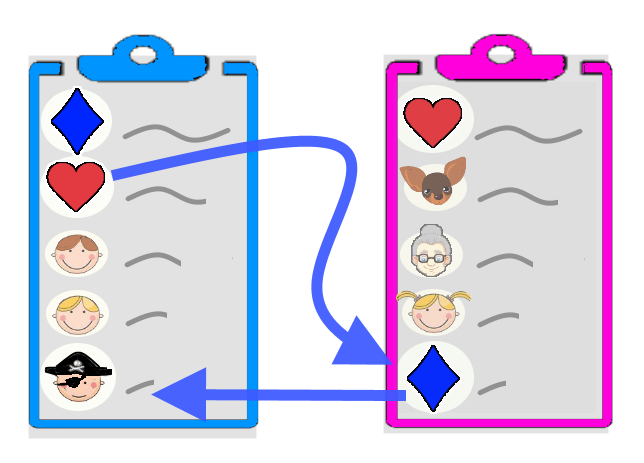
\includegraphics[width=0.5\linewidth]{pdn_reciprocity.png}}
    \caption{The blue list has a red heart as 2nd. Dog is opposite to it. The pink list has a blue diamond as 5th the same rank as the pirate.} \label{fig:Reciprocity}
\end{figure}

Here comes the reality.
You are the fifth on the list. Same as the beggar on your list?
You should treat her accordingly (this is not a relationship advice).
\\She can reverse the evaluation by multiplying the relationship by rank's ratio you to dog (5 over 2).

\subsection{Quantum “density”}\label{Density}
\epigraph{What comes first thought or being?}{The fundamental question of philosophy}

The famous experiment\cite{Dualism} with cannon firing particles through two slits draws not two stripes but a zebra of interference. It is as if the gun is charged not with a particle but with a liquid passing simultaneously through both slits. The particle behaves like a wave (wave-particle dualism). We propose a solution to this contradiction by shifting the focus from the observer selecting the observed object to the space.

% https://tex.stackexchange.com/questions/37581/latex-figures-side-by-side
% http://www.peteryu.ca/tutorials/publishing/latex_captions
\begin{figure}[!htb]
  \begin{minipage}[c]{0.40\linewidth}
    \href{\githubPics pdn_double_slit1a.png}{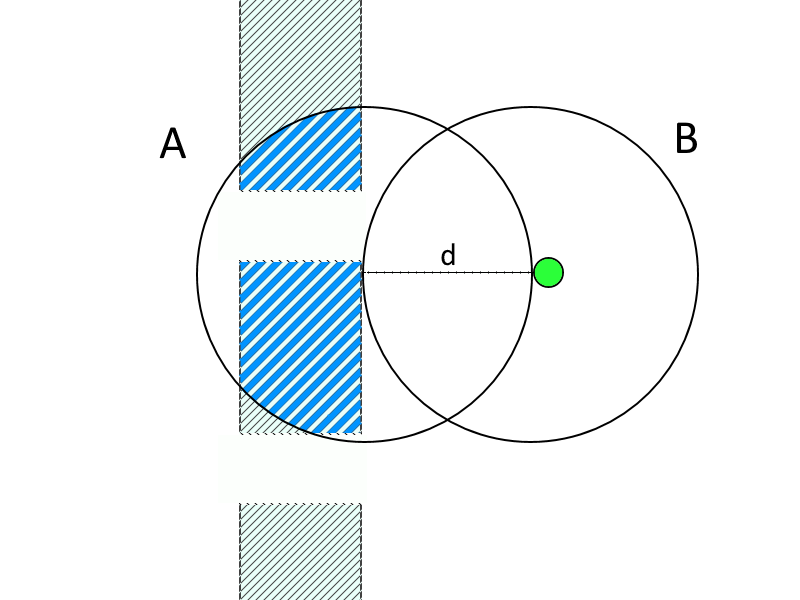
\includegraphics[width=\linewidth]{pdn_double_slit1a.png}}
    \subcaption{Sphere A covered one slit.}
  \end{minipage}\hfill
  \begin{minipage}[c]{0.40\linewidth}
    \href{\githubPics pdn_double_slit1b.png}{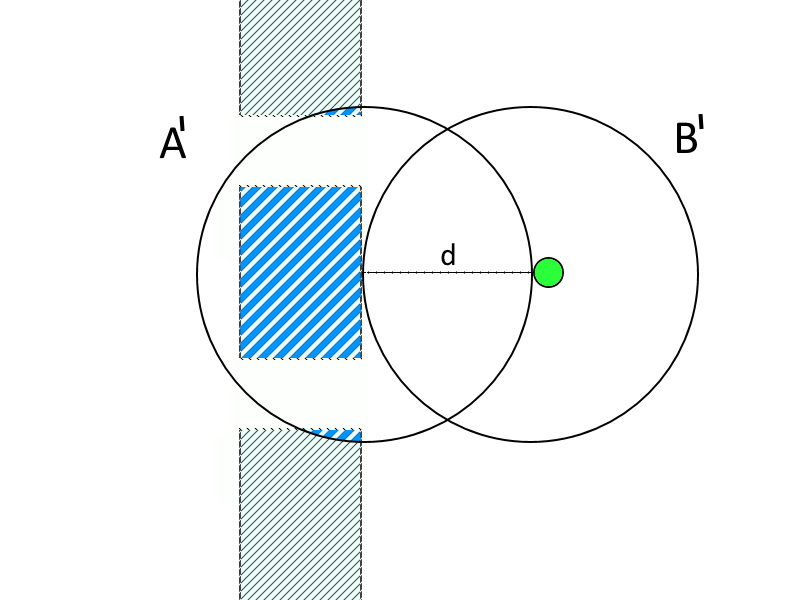
\includegraphics[width=\linewidth]{pdn_double_slit1b.png}}
    \subcaption{Sphere A' covered two slits.}
  \end{minipage}
  \caption{Wall with two slits and green projectile. Spheres A and A' differs by “density”. Spheres B and B' are identical.} \label{fig:DoubleSlit}
\end{figure}

Figures~\ref{fig:DoubleSlit} show two cases where a particle (green ball) is in different positions relative to the slits but at the same distance from the wall. Assuming space as the center, we obtained two intersecting spheres. Let us consider the "densities" of spheres in different cases. The right spheres B and B' are identical. However, sphere A contained more substance than sphere A'. Centricity on space will take into account this difference and will open the possibility of comparing these cases.

\begin{figure}[!htb]
  \begin{minipage}[c]{0.40\linewidth}
    \href{\githubPics pdn_double_slit2a.png}{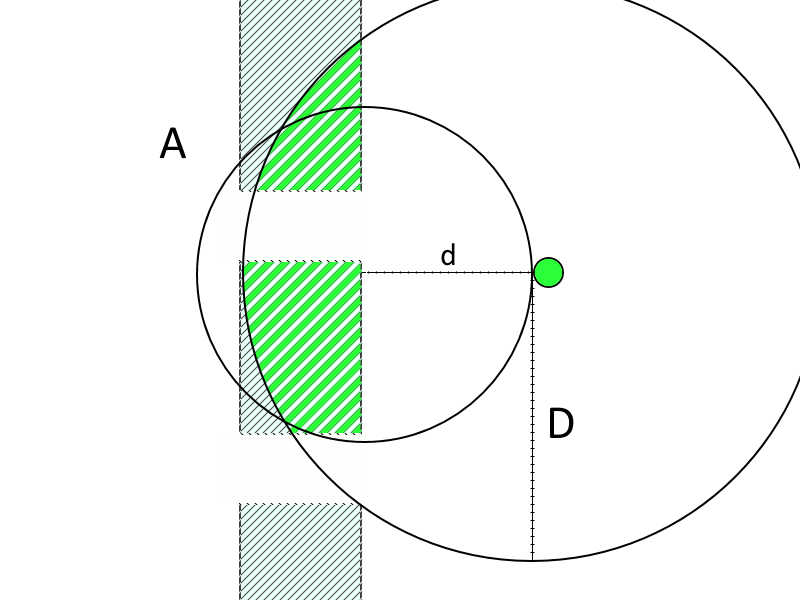
\includegraphics[width=\linewidth]{pdn_double_slit2a.png}}
    \subcaption{The growth of D hit the emptyness of bottom slit.}
  \end{minipage}\hfill
  \begin{minipage}[c]{0.40\linewidth}
    \href{\githubPics pdn_double_slit2b.png}{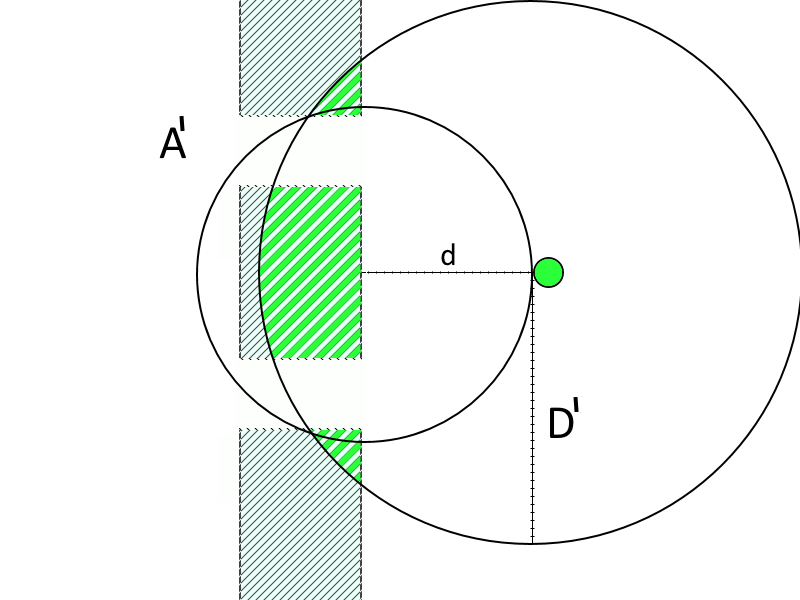
\includegraphics[width=\linewidth]{pdn_double_slit2b.png}}
    \subcaption{The growth of D' devoured both walls outside of A'.}
  \end{minipage}
  \caption{Blue area of previous figures equal to a green area, e.g. substance areas A=D and A'=D'. And radius D > D'.} \label{fig:DoubleSlit2}
\end{figure}

Distance $d$ is not suitable for measuring the space between the sides, as it does not reflect the difference in the amount of substance. To find the dialectical distance that considers the substance of both sides, it is necessary to increase the radius of sphere B to the level of the substance in sphere A. Similarly, the same is true for sphere B' (Fig.~\ref{fig:DoubleSlit2}). The dialectical distances and quantities of substance differ, and hence the "forces" in each case are also different.
\\The proposed interaction is not the purpose of this study and is only a demonstration of the consideration of the priority of matter-space over consciousness-observer.

\[ \triangle \]

These examples show how to dialectically resolve dependence on the observer. The examples were analyzed analytically: two opposite sides were discovered, and a solution was made that included both sides. However, where do we obtain opposites for analysis if an abstract problem is solved in general? The self-development of categories gives rise to their opposites. The "not" particle will allow us to synthesize the next step of the process. It will turn out that new is based on the old, and there will be no room for the observer.

\subsection{The singular and the contradictions}
\epigraph{There is only one subject, the~world~as~a~entirety.}{Basis of dialectical materialism}

The space exist. The space is everything. The space is one.
\\\textit{Not} space is nothing. \textit{Not} everything is nothing. There are many nothings.
\\\textit{Not} everything-nothing are the holes in the space, called points. A point itself is nothing. Only the relations to other points puts meaning into it. 

The relation of a point to another point is the direction that captures and bounds a part of space. Such a subject-object relation can be represented as a space-sphere with a center-subject and a radius-direction to the object. Space-sphere will bound $\overrightarrow{r_{s}}$ points, this is a quantitative property of the relation. \textit{Not} quantitative is a qualitative property -- it is the "radius", the distance from the subject to the object. Quantity and quality are inseparable and together form the quantitative-qualitative (hereinafter referred to as q-q) properties of the relation of the subject $s$ to the object:
\begin{align*}
\overrightarrow{r_{s}} \cdot d_{s}(\overrightarrow{r_{s}})
\end{align*}

\textit{Not} subject-object relation is an inverted relation, that is object-subject relation. Such relation with the direction from the object, but with the preservation of the centrality of the subject. The space-sphere is quantitatively shifted into an object, but qualitatively remains in the subject (see Fig.~\ref{fig:Points}). The inverse quantity is formed by an external count, and the quality is a function of this quantity. The subject is reflected in the object, and receives a distorted picture of reality. The relation of the object to the subject $s$:

\begin{align*}
\overleftarrow{r_{s}} \cdot d_{s}(\overleftarrow{r_{s}})
\end{align*}

\begin{figure}[H]
  \centering
  \href{\githubPics pdn_reverse_vector.png}{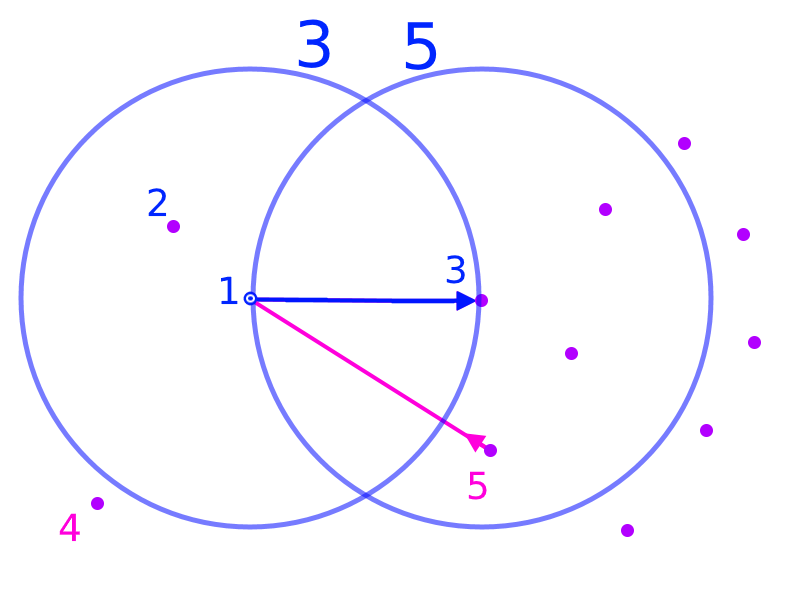
\includegraphics[width=0.8\linewidth]{pdn_reverse_vector.png}}
  \caption{The subject number 1. The object number 3. In the subject's (left) sphere there are 3 points, in the object's (right) sphere there are 5 points. The new inverted pink 5-radius is larger than the initial blue 3-radius.}\label{fig:Points}
\end{figure}

\textbf{Opposites}. For the subject $s$, one relation to the object is two opposite expressions mediated by space:
\begin{align*}
  \overrightarrow{r_{s}} \cdot d_{s}(\overrightarrow{r_{s}}) \quad &\textit{vs} \quad  \overleftarrow{r_{s}} \cdot d_{s}(\overleftarrow{r_{s}}) 
  \end{align*}

There are many such relations for each subject and the subjects themselves are also many. For further development, the plurality must be removed. \textit{Not} the plurality of relations is a particular relation, the closest. In order to find such a relation, it is necessary to lift three moments: singularity, universality and particularity. 

\textbf{Measure}. The measure clears quality of quantity and allows us to compare opposites. Mathematically, this means that pairs of numbers will be reduced to single values. Pairing prevents comparison (it cannot be answered what pair is greater (2; 1.5) or (3; 1)). Pairs of q-q must be reduced to single qualities, for this we divide both sides by the number of points from the (right) object part. \textit{Not} quantity-quality are the measures of the subject-object relations
\begin{align*}
\frac{\overrightarrow{r_{s}} \cdot d_{s}(\overrightarrow{r_{s}})} {\overleftarrow{r_{s}}} \quad &\textit{vs} \quad \frac{\overleftarrow{r_{s}} \cdot d_{s}(\overleftarrow{r_{s}})} {\overleftarrow{r_{s}}}
&\intertext{or}
\frac{\overrightarrow{r_{s}} } {\overleftarrow{r_{s}}} \cdot d_{s}(\overrightarrow{r_{s}}) \quad &\textit{vs} \quad d_{s}(\overleftarrow{r_{s}})
\end{align*}

\textbf{Totality}. The greatest (universal) of the measures will satisfy the "densities" of both sides.
\begin{align*}
  \max(\frac{\overrightarrow{r_{s}} } {\overleftarrow{r_{s}}} \cdot d_{s}(\overrightarrow{r_{s}})&; \quad d_{s}(\overleftarrow{r_{s}}))
  \end{align*}

The opposites within the relation are resolved, but the oppositions of the plurality remain.

\textbf{Assertion}. The second negation of plurality is to find the smallest (particular) of all relations. What produces the abstract universal

\begin{align}
  \min_s( \max(\frac{\overrightarrow{r_{s}}} {\overleftarrow{r_{s}}} \cdot d_{s}(\overrightarrow{r_{s}}) ; d_{s}(\overleftarrow{r_{s}}))) = RD \label{formula:BorderRD}
\end{align}

The first phase ended with the unity of opposites. The points limited the space and produced a piece of space. The space cranked through and lifted itself of the points, of their subjectivity and directionness. The next phase is coming, in which we will deal with the groups and the becoming of clusters.

\textbf{Restart the process}. As we shall learn later, it was not the points that cut off the space, but the groups through the points. Therefore, when restarting the process of finding the smallest relation, it is necessary to take into account the belonging of points to groups. Eventually, all points will come together into one community, which can be represented by a spanning tree\cite{strMST}.

\textbf{Orderliness of connections}. The process sorts the connections, befriends the same densities, delays the addition of outliers. Using Fig.~\ref{fig:OrderSquare} as an example, all points are equidistant from each other, but nevertheless, the body and edges will connect first, and the vertices at the very end. For the same "density", the distances are approximately equal to. For regions with different "densities" $\overrightarrow{r} \neq \overleftarrow{r} $ and $d(\overrightarrow{r}) \neq d(\overleftarrow{r})$, which reduces the order. For outliers $r = 2$, priority as last.

\begin{figure}[H]
  \centering
  \href{\githubPics pdn_square_order.png}{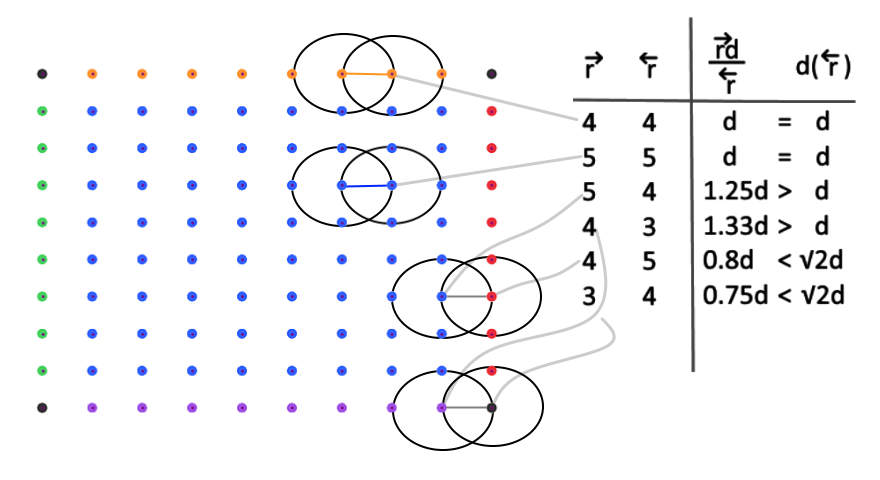
\includegraphics[width=0.8\linewidth]{pdn_square_order.png}}
  \caption{Values of ranks and distances in ascending order: equidense core and edges, then core-edges, last vertex outliers.}\label{fig:OrderSquare}
\end{figure}


\section{Dialectics of Negation}
\epigraph{Struggle and unity of opposites.}{Law of dialectics}

The particle "not" made it possible to unfold the internal contradictions of space. Such negation reveals the distinctions of the moments and drives the process forward toward self-return. This negation lies at the heart of dialectical development.

However, some negations can be destructive. Like negation of a bug -- is swapping it dead. Or it can be an everything-but type. This is similar to subtraction of an element from a mathematical set. These kinds of negations are dead, they will not produce any development, and further negation is spoiled. In contrast, dialectical negation remains in the context of the negatee and yet produces a higher-level entity. Like fixing the bug in the code.

Advancement to a higher level does not bring anything from the outside. Hegel's System of Logic starts from Nothing-Being-Becoming, advances through Quantity-Quality-Measure, and leads to the highs of the Absolute. All the advancements came from within, and the Absolute was only hiding in the Nothing. In the present work, contamination with external ideas was similarly prevented, but the reflections were made against real Beings and not off the \textbf{idea}listic Absolute.

Hegel's narration creates distinct negation triads and their inner structure discussed with analysis of the \textit{moments}. It is not possible to fit a triad-centric approach into the formula; that is, where another thinker comes along. Mao Tse-tung in his work "On Contradiction"\cite{OnContradiction} highlighted the role of the opposites in numerous examples, that lead to math friendly opposite-centric result. Mao's quote precisely describes the emergence of a cluster: "It holds that external causes are the condition of change and internal causes are the basis of change, and that external causes become operative through internal causes."\cite{OnContradiction}.

In brief, as Lenin wrote, dialectics can be defined as the doctrine of the unity of opposites\cite{PhilisophicalNotebooks}. To proceed further in the study of dialectics, we recommend starting with Stalin's work "Dialectical and Historical Materialism,"\cite{HistoricalDiaMat} which unrolls the epigraphs of the present work in an easy-to-read manner.

\section{The particular and the substance}
\epigraph{Transition of quantitative changes into~qualitative~changes.}{Law of dialectics}

In the first phase, the singulars cut off a piece of space (RD\eqref{formula:BorderRD}). This result is an abstract universal. And for each of the two adjacent points, it is the absolute universal, their definitive border. Such is the end of the second phase. Subsequently, the merge into the group will follow, and at the restart of the process, there will be a group of two clusters defined by the RD border. This is a naive process for the initial formation of groups.
% Revealed doesn't mean to be known.

\textbf{Opposites}. In the later restarts, the groups and not the points are connected. The external abstract universality RD will collide with already accepted internal absolute universals. There are a plurality of opposites of external and internal:
\\ $RD \quad vs \quad k_i \cdot g_i$, where $k_i \cdot g_i$ is q-q of cluster $i$ in one of the groups.

Each cluster has this relation. Clusters are parts of a group. This lack of unity is solved by lifting three moments: particularity, singularity and universality.

\textbf{Measure}. We bring external to the internal quantity of the cluster, thereby lifting the quantitative particularity.
\begin{align} 
  \frac { RD } {k_i} \quad &\textit{vs} \quad \frac { k_i \cdot g_i } {k_i} \notag
  \intertext{or} \notag
  RD \frac { 1 } {k_i} \quad &\textit{vs} \quad g_i \notag
\end{align}

\textbf{Totality}. The sum(singular) collects the clusters and their reflections into a single ones:
\begin{align*}
  RD \sum_{K} { \frac { 1 } {k_i}} \quad &\textit{vs} \quad \sum_{K} { g_i }
\end{align*}

\textbf{Assertion}. It turned out to be a confrontation between the whole and parts. The greatest(universal) of the parties shows the appearance of the group and its q-q properties: 
\begin{align} \label{formula:AppearanceKG}
  KG = \max (RD \sum_{K} { \frac { 1 } {k_i}} \quad &; \quad \sum_{K} { g_i }) 
\end{align}

If the new wins, then the border transitions into a group and a cluster\footnote{In Hegelian terms, cluster is substance and group is substrate.} with q-q properties $ KG~=~RD \sum_{K} { \frac { 1 } {k_i}} $ is born. If the old stands, the border is ignored.

\textit{Essentially, the clustering formula tests whether the new distance can overcome the old cluster structure minus the dilution by outliers.}


\textbf{Restart the process}. For further confrontations, the newly formed cluster carries $G~=~RD \cdot avg { \frac { 1 } {k_i}} $ (average internal structure), and on the opposite hand $\frac { 1 } {K}$. The more complex the structure of the cluster, the more difficult it will be to reform.

\textbf{Outliers}. Clusters with $k_i = 1$  significantly boost $RD \sum_{K} { \frac { 1 } {k_i}} $, that is, the chance of clustering.

\textbf{Isolation of the sides of the connection}. The $RD$ border independently affects both sides of the connection. There are three possible outcomes: 2, 1, or 0 clusters per connection.

\section{The universal and the merge}

\epigraph{Negation of the negation.}{Law of dialectics}

In the first phase, space substantiates itself by means of groups. In the second phase, this external substantiated the two groups. The two parts assert themselves and their appearances. These are now available to each other for merging. Their merger gave rise to a new state of the entire system.

Restarting the entire algorithm with new groups, produces a new merge. And so, over and over again, the separate groups will be uniting until total unity. The end of Druhg clustering interrupts the development.

However, the dialectic of negation knows no end. Having come to the impossibility of development, there will be negation of the entire system. The tick of time restarts the self-development of space with displaced points. The displacement phase was derived from the cyclic symmetry of the conclusion figures (see Table~\ref{table:Phases}). The conclusions are the most ordinary relations of things~\cite{PhilisophicalNotebooks}. The rose is a plant; the plant needs moisture; therefore, the rose needs moisture, i.e. the rose, as a singular, closes through the particular, with the universal~\cite{ScienceOfLogic3}. 

We observed similar closures of moments in the first phase: the subject-object converged in one relation, and through these relations, one was found. That is, the U-universality united in the S-singular (U-S), and from the S-singulars the P-particular stood out (S-P). Again, the result has all three moments, S-U-P, but already as particular. Therefore, the following conclusion shifts to S-P and P-U. For the third phase, P-U and U-S, the removed directionness returns, and the points shift to the group centers. Let us consider the implementation of this forecast at another time.

  \begin{table*}
    \centering
    \resizebox{\linewidth}{!}{%
    \begin{tblr}{
      width = \linewidth,
      colspec = {Q[58]Q[160]Q[71]Q[144]Q[75]Q[63]Q[79]Q[162]Q[117]},
      cells = {c,m},
      cell{1}{1} = {r=2}{},
      cell{1}{2} = {r=2}{},
      cell{1}{3} = {r=2}{},
      cell{1}{4} = {r=2}{},
      cell{1}{5} = {c=3}{},
      cell{1}{8} = {c=2,r=2}{},
      cell{3}{1} = {r=2}{},
      cell{3}{4} = {r=2}{},
      cell{4}{8} = {c=2}{},
      cell{5}{1} = {r=2}{},
      cell{5}{4} = {r=2}{},
      cell{6}{8} = {c=2}{},
      cell{7}{1} = {r=2}{},
      cell{7}{4} = {r=2}{},
      cell{8}{8} = {c=2}{},
      vline{2,5,8} = {-}{},
      hline{1,3,9} = {-}{0.12em},
      hline{5,7} = {-}{},
    }
    \begin{sideways}\textbf{Phase}\end{sideways}   & \textbf{Reflection environment}  & \textbf{Subject~}  & \textbf{~Opposites}                          & \textbf{Conclusion} &          &           & \textbf{Result}              &                       \\
            &                         &          &                                    & \begin{sideways}\textbf{Measure}\end{sideways} & \begin{sideways}\textbf{Totality}\end{sideways} & \begin{sideways}\textbf{Assertion}\end{sideways} &                          &                       \\
    I  & Space                   & Points   & {$\overrightarrow{rd}$ \textit{vs} $ \overleftarrow{rd}$ \\Subject object }    & 1/r        & max      & min       & Connection of Groups     & Border RD~\eqref{formula:BorderRD}             \\
            & U                       & S        &                                    & S          & U        & P         & P                        &                       \\
    II & Group of Connection     & Clusters & {RD \textit{vs} kg\\External internal } & 1/k        & sum      & max       & Clusterization           & Appearance KG (~\eqref{formula:AppearanceKG})        \\
            & S                       & P        &                                    & P          & S        & U         & U                        &                       \\
    III     & Cluster                 & Groups   & KG \textit{vs} nv                           & 1/n        & min      & sum       & Attraction repulsion & {Center NV} \\
            & P                       & U        &                                    & U          & P        & S         & S                        &                       
    \end{tblr}
    }
        \caption{ The project of the scheme of the full automata. U~-~universality, P~-~particularity, S~-~singularity} \label{table:Phases}
    \end{table*}



\section{Experiments}\label{Examples}
\epigraph{Practice is the criterion of Truth}{Karl Marx, Theses On Feuerbach, 1845}

\textbf{Data Sets.} We report the performance on toy sklearn, Chameleon, and synthetic geometric datasets. We used Euclidean distance for all of them.
\\ \textbf{Algorithm.} The code is publicly available (https://github.com/artamono1/druhg) and can be run on several lines of code. The pseudocode is given in Appendix \ref{Pseudocode}. The tests were conducted on the Python version of \textit{druhg 1.5.0}.

Druhg does not require parameters, unlike other algorithms. The current implementation uses a KD-tree with k-neighbor limitations for a performance boost. A gap and an outlier can equally trigger clustering, which can lead to global outlier clustering of the entire dataset. The user can pick the desired scale of cluster sizes without rerunnig the main algorithm.


\subsection{Performance and precision}

\begin{figure}[!htb]
  \centering
  \href{\githubPics run_diffNNs.png}{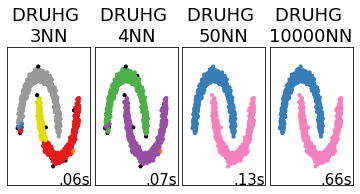
\includegraphics[width=0.8\linewidth]{run_diffNNs.png}}
  \caption{Low k-nn doesn't include moon connections. Higher k-nn takes longer.} \label{fig:DifferentNN}
\end{figure}

(Fig.~\ref{fig:DifferentNN}) The Underlying KD-tree uses the k-near-neighbor parameter. The greater the \textit{k}, the more precise the result for the price of performance. 
After some \textit{k} the result won't change.


\subsection{Hierarchy and size filter}

Run it once to build a hierarchy of clusters. 
Usual way of filtering is a providing a max distance parameter. We propose a new way of accessing hierarchy tree, by limiting the max size of the cluster (see Fig.~\ref{fig:Chameleon}).

\begin{figure}[!htb]
  \begin{minipage}[c]{0.40\linewidth}
    \href{\githubPics run_chameleon05.png}{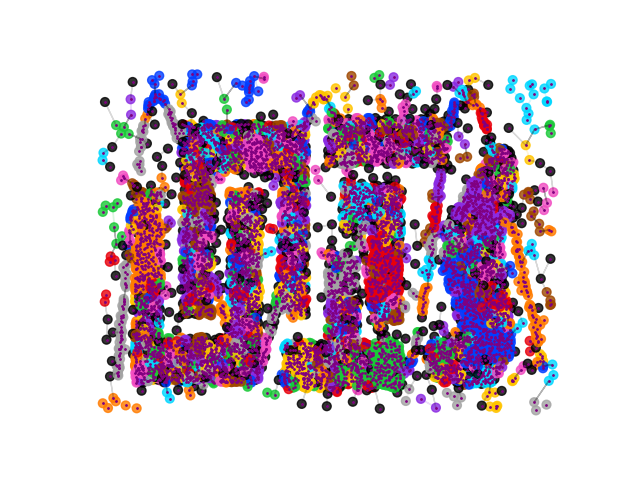
\includegraphics[width=\linewidth]{run_chameleon05.png}}\caption*{5\%}
  \end{minipage}
  \begin{minipage}[c]{0.40\linewidth}
    \href{\githubPics run_chameleon25.png}{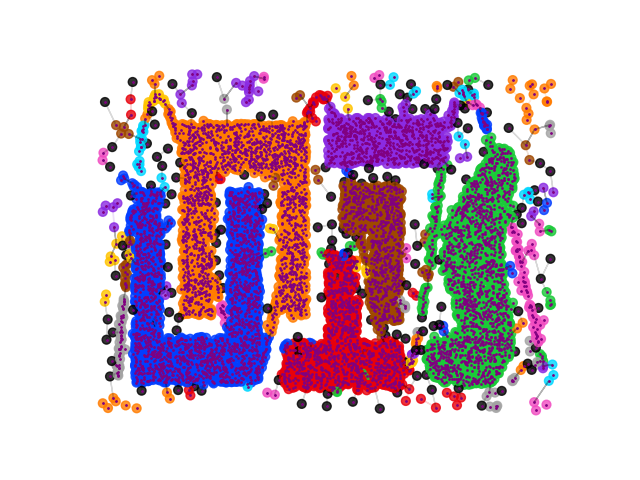
\includegraphics[width=\linewidth]{run_chameleon25.png}}\caption*{\underline{25\%}}
  \end{minipage}
  \begin{minipage}[c]{0.40\linewidth}
    \href{\githubPics run_chameleon45.png}{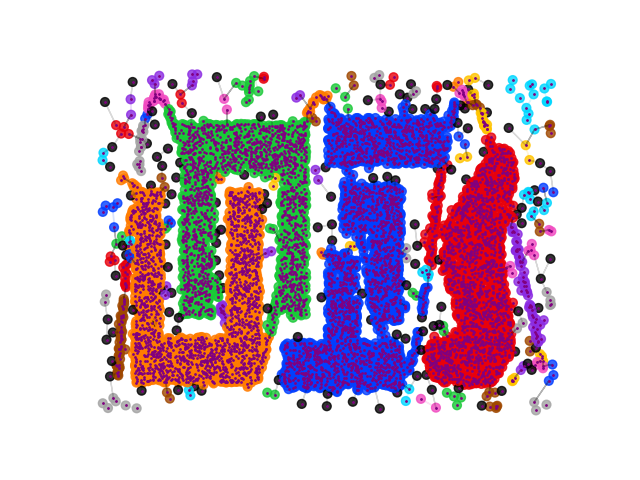
\includegraphics[width=\linewidth]{run_chameleon45.png}}\caption*{45\%}
  \end{minipage}
  \begin{minipage}[c]{0.40\linewidth}
    \href{\githubPics run_chameleon75.png}{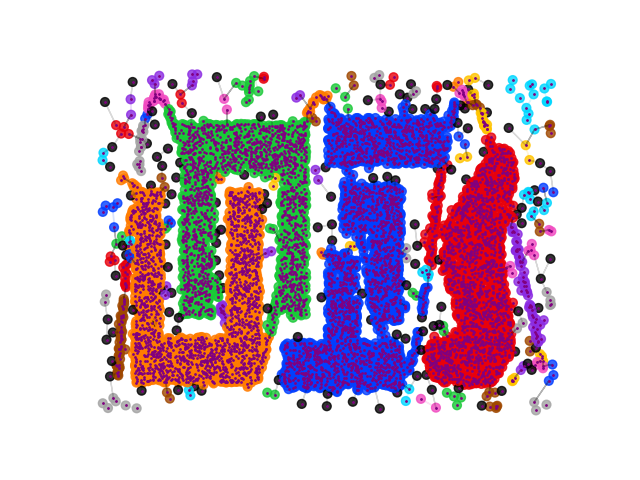
\includegraphics[width=\linewidth]{run_chameleon75.png}}\caption*{75\%}
  \end{minipage}
  \begin{minipage}[c]{0.40\linewidth}
    \href{\githubPics run_chameleon100.png}{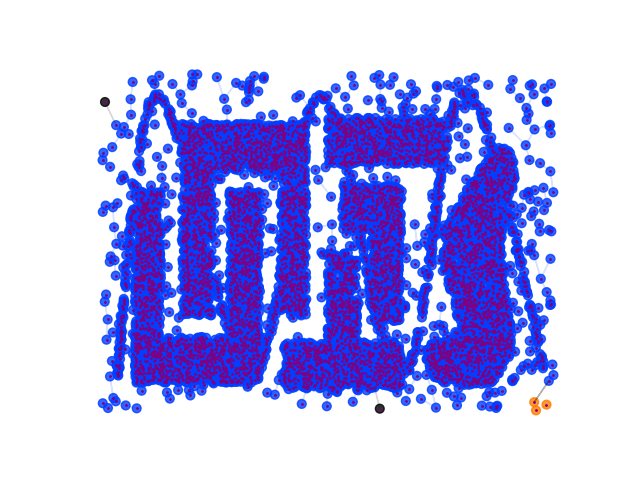
\includegraphics[width=\linewidth]{run_chameleon100.png}}\caption*{100\%}
  \end{minipage}
  \caption{Chameleon dataset. One Druhg run. Relabel function with X\% top cluster limit.} \label{fig:Chameleon}
\end{figure}

\subsection{Basic shapes}

\begin{figure}[!htb]
  \begin{minipage}[c]{0.20\linewidth}
    \href{\githubPics pdn_line.png}{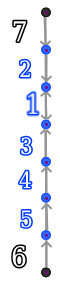
\includegraphics[width=0.4\linewidth]{pdn_line.png}}
  \end{minipage}\hfill
  \begin{minipage}[c]{0.40\linewidth}
    \href{\githubPics pdn_square.png}{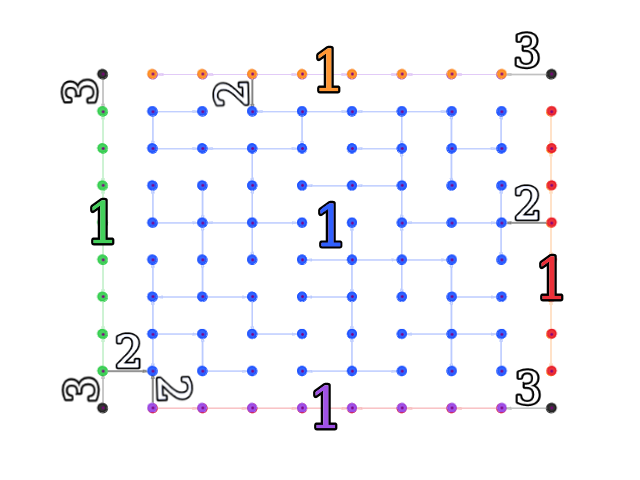
\includegraphics[width=\linewidth]{pdn_square.png}}
  \end{minipage}\hfill
  \begin{minipage}[c]{0.40\linewidth}
    \href{\githubPics run_cube.png}{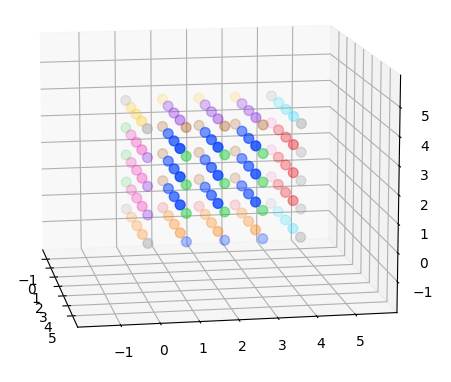
\includegraphics[width=\linewidth]{run_cube.png}}
  \end{minipage}
  \caption{Order of connections for the basic shapes of equidistant grid points.} \label{fig:Geoshapes}
\end{figure}

(Fig.~\ref{fig:Geoshapes}). First, the same density points connect to produce dense bodies (marked in blue). These links are cluster deterministic, and a change in the first point does not change the end clustering result. The results are scale independent.
Druhg defined vertexes, edges, and faces, similar to humans. 

\subsection{Comparison with others}
\begin{figure}[H]
  \centering
  \href{\githubPics run_comparison.png}{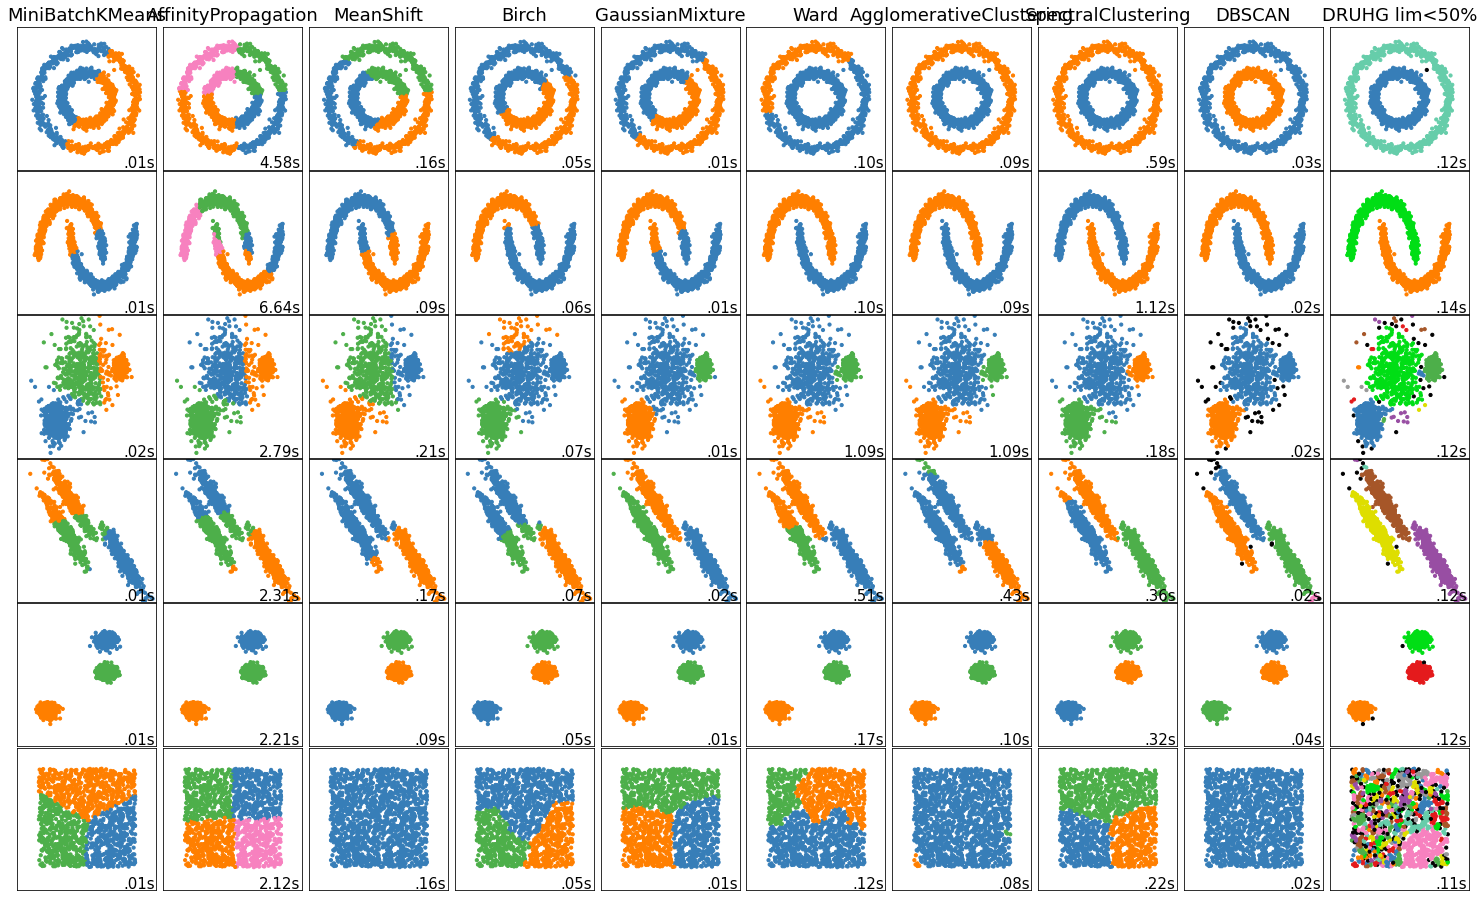
\includegraphics[width=0.8\linewidth]{run_comparison.png}}
  \caption{Toy sklearn datasets comparison. Last column is Druhg.} \label{fig:SklearnDatasets}
\end{figure}

(Fig.~\ref{fig:SklearnDatasets}) Druhg managed to catch individual global outliers and small clusters in the first run. Some algorithms outperform Druhg by knowing their exact parameters in advance.
The bottom-right corner chaos highlights the philosophic core of the algorithm -- it is not possible to define Being without Other.

% MedMNIST v2 ???

\subsection{The critical point}

\begin{figure}[!htb]
  \centering
  \href{\githubPics pdn_sandpiles.png}{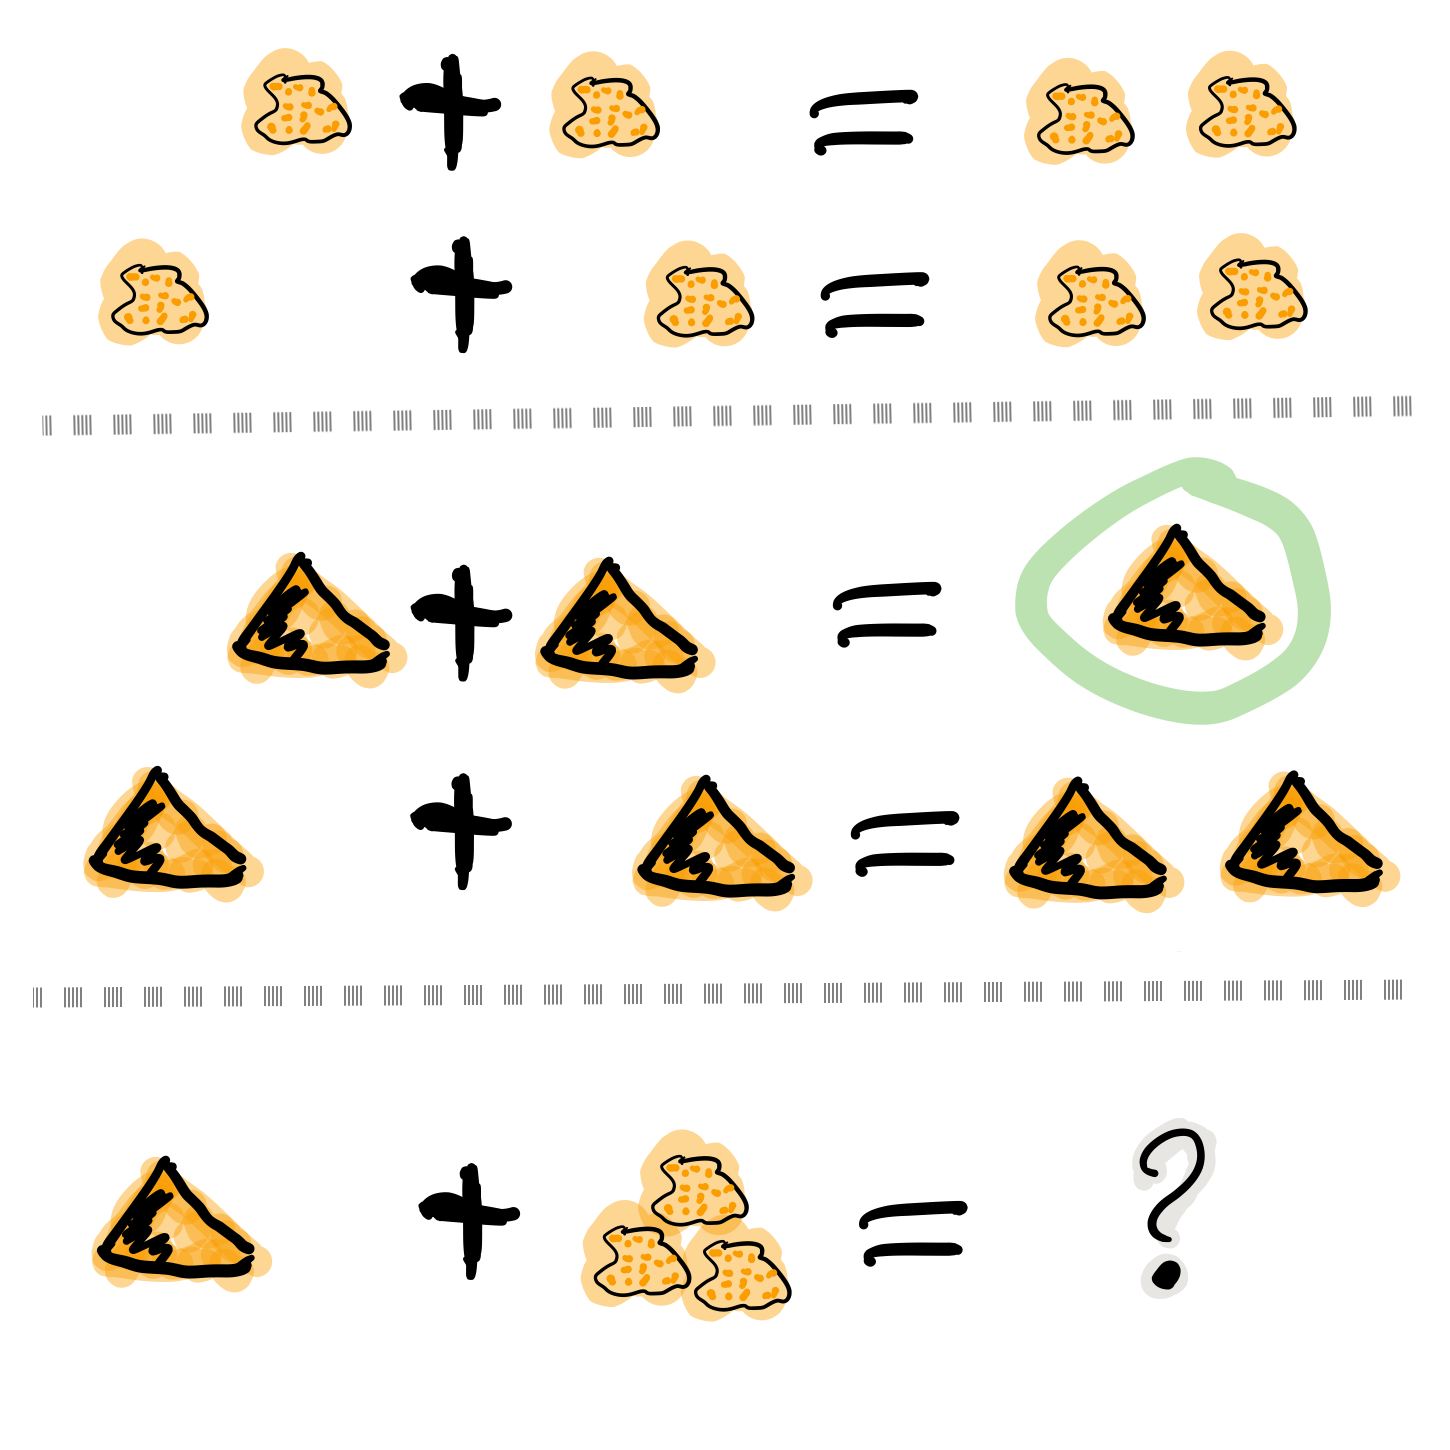
\includegraphics[width=0.5\linewidth]{pdn_sandpiles.png}}
  \caption{Sandpiles and sandgrains aggregations with varying distances.}\label{fig:Sand}
\end{figure}
(Fig.~\ref{fig:Sand}) When does a pile become a pile? The thousands year question might be answered by Druhg.

\section{Final remarks}
\epigraph{\raggedleft So many blissful revelations
\\Drawn by enlightenment's thought:
\\And skill, the son of toughest errors,
\\And genius, the paradoxes' pal,
\\And chance, the god-inventor.}{Alexander Pushkin, 1929}

A new clustering approach was introduced that provides: (i) a complete density-based clustering hierarchy; (ii) does not require parameters; (iii) a choice of metric defines near distances, that develop everything else. The philosophical narrative was led through dialectics, and the cluster was defined. Experiments on various datasets showed the SOTA results. This work opens up a wide range of opportunities for future research: performance evaluation and improvement; discovery of the properties of dialectical distance and spanning tree; the birth of the displacement of points in the third phase, and the construction of a quantum-qualitative model.


%%%%%%%%%%%%%%
% References %
%%%%%%%%%%%%%%

\newrefcontext[sorting=ynt]
\printbibliography
\onecolumn

%%%%%%%%%%%%
% Appendix %
%%%%%%%%%%%%

\begin{appendices}
\section{Pseudocode}\label{Pseudocode}
% мануал по псевдокоду http:\\mirror.ox.ac.uk/sites/ctan.org/macros/latex/contrib/algorithmicx/algorithmicx.pdf

DRUHG(\foreignlanguage{russian}{drug}): Dialectical Reflection Universal Hierarchical Grouper.
\\ The algorithm consists of two parts: Tree building and cluster detecting/labeling.

The Tree is stored with union-find data structure aka merge-find set.\cite{strUF}
\\ The neighbors are found with KD-tree\cite{strKDtree} which allows to access k near neighbors. Keep in mind, that large k-near-neighbors parameter doesn't contribute to precision, but slows down the executions.

\begin{algorithm}
  \begin{algorithmic}[1]
    \Procedure {Pure reciprocity}{$Points$}: \Comment Adding pure reciprocal relation to the tree
      \ForAll {$p \in Points$}:
        \If {p's nearest neighbor has p as it's nearest}:
            \State Add the edge to the Tree 
            \State Weight = distance
        \EndIf
      \EndFor
    \EndProcedure
    \algstore{bkbreak}
  \end{algorithmic}
  \end{algorithm}

Although we are looking for a global optimum, in practice the subtrees start to grow from those 1-on-1 connections. Those connections always precedes everything else. Even thou global order would be broken. 
\\ In a sense algorithm is location-independent and separate Trees could be grown for a speed up. 

  \begin{algorithm}[h]
    \begin{algorithmic}[2]
      \algrestore{bkbreak}
      \Procedure {BuildMST}{$Points$}: \Comment Find minimal edge and connect to the Tree
        \Repeat
          \State \textit{GlobalMinimum} = INF
          \State \textit{GM-Edge} = Null
          \ForAll {$p \in Points$}:
            \ForAll {$nn \in p's$ neighbors}:
              \If {\textit{p} and \textit{nn} are connected(same subtree)}:
                \State pass
              \EndIf
              \State \textit{d} = distance to the \textit{nn} in \textit{p}'s POV
              \If {\textit{d} > \textit{GlobalMinimum}}:
                \State \indent derivative \textit{DialecticValue} always greater than \textit{d}
                \State break
              \EndIf

              \State \textit{r} = rank of the \textit{nn} in \textit{p}'s POV
              \State \textit{R} = rank of the \textit{p} in \textit{nn}'s POV
                
              \If {$r > R$}:
                \State pass
              \EndIf
              \State \textit{DialecticValue} = $min(D; \frac{R \cdot d}{r})$:
                \State \indent \textit{DialecticValue} includes POV of both points
                \State \indent \textit{D} = distance to the \textit{R} in \textit{p}'s POV
              \If {\textit{DialecticValue} < \textit{GlobalMinimum}}:
                \State \textit{GlobalMinimum} = \textit{DialecticValue}
                \State \textit{GM-Edge} = (\textit{p}, \textit{nn}, \textit{DialecticValue})
              \EndIf
            \EndFor
          \EndFor
          \State Add \textit{GM-Edge} to the Tree
        \Until{all edges are connected in one tree}
        \State
        \Return {The Tree: ordered edges and weights}
      \EndProcedure
    \algstore{bkbreak}
\end{algorithmic}
\end{algorithm}

The $O(n^2)$ time complexity, can be improved. The \textit{DialecticValue} is monotonically growing for every points and outside loop can be fixed with a heap\cite{strHeap} structure.
\\ Those improvements decreases time complexity significantly.

\begin{algorithm}[h]
  \begin{algorithmic}[3]
    \algrestore{bkbreak}
      
    \Procedure {LabelClusters}{$Tree$}: \Comment Labeling subtrees as clusters
      \State Inners(p) = 0
      \ForAll {edge(pair, weight) in Tree}:        
        \For {Left and Right subtrees}:
            \State \textit{Border} = weight $\cdot \sum{\frac{1}{k_i}}$:
            \State \indent $k_i$ = amount of clusters in subtree
            \State \textit{Inners} = $\sum{g_i}$:
            \State \indent $g_i$ = quality of cluster in subtree
            \If {\textit{Border} $>$ \textit{Inners}}:
              \State *That subtree is a cluster*
              \State It's $k_i \cdot g_i $ = \textit{Border}
            \EndIf
        \EndFor
        \State Merge subtrees: 
        \State \indent Add sizes and qualities, numbers of clusters and points
      \EndFor
    \EndProcedure
  \end{algorithmic}
\end{algorithm}

Labeling is straight O(n) forward.
\section{Translation}
Translation in Russian is available\cite{Druhg_ru}.
\end{appendices}

\end{document}

% Create PDF on Linux:
% FILE=test; pkill -9 -f ${FILE} &>/dev/null; rm -f ${FILE}*aux ${FILE}*bbl ${FILE}*bib ${FILE}*blg ${FILE}*log ${FILE}*out ${FILE}*pdf &>/dev/null; pdflatex -halt-on-error ${FILE}; bibtex ${FILE} && pdflatex ${FILE} && pdflatex ${FILE} && (xdg-open ${FILE}.pdf &)